\newpage
\appendix
\onecolumn
\begin{center}
	\textbf{\LARGE Appendix }
\end{center}

% \begin{center}
% 	\textbf{\large Concept-based Explanations for Out-of-Distribution Detectors}
% \end{center}
In Section~\ref{sec:app_discussion}, we discuss additional aspects of our method such as the choice of auxiliary OOD dataset, human subject study, and societal impact.
In Section \ref{sec:appendix-A}, we discuss the connection of the proposed concept separability to Bhattacharya Distance, and the per-class variations of detection completeness and concept separability, followed by the overall algorithm for concept learning.
In Section \ref{sec:appendix-implementation-details}, we provide the detailed setup for the experiments and additional thorough analysis of our concept learning objective.
In Section \ref{app:auxiliary-ood}, we discuss whether our concept learning objective remains effective even when a synthesized auxiliary OOD dataset similar to target ID data is used.
In Section \ref{sec:appendix-shapleys}, we illustrate additional examples of our concept-based explanations.


% short analysis of the ConceptSHAP in the appendix like Yeh et al do
% Connection to dimensionality reduction, Fisher's score?
\section{Discussion and Societal Impact}
\label{sec:app_discussion}
\mypara{Auxiliary OOD Dataset.} 
%Our approach also remains a limitation in that an auxiliary dataset of an OOD distribution is required.
A limitation of our approach is its requirement of an auxiliary OOD dataset for concept learning, which could be hard to access in certain applications.
% A weakness of our approach is that it requires an auxiliary OOD dataset for concept learning. 
% Unfortunately, access to such data could be a luxury in certain applications.
To overcome that, a research direction would be to design generative models that simulate domain shifts or anomalous behavior and could create the auxiliary OOD dataset synthetically, allowing us additional control on the extent of distributional changes the resulting concepts could deal with (see Appendix~\ref{app:auxiliary-ood} for further discussion). 

% We believe this work takes a step toward building trust in the deployment of OOD detectors, which will help the practical integration of such systems towards making societal decisions.

\mypara{Human Subject Study.} 
% One would suggest performing a user study to get a more extensive understanding of the effectiveness of our method in the hands of ML practitioners.
Performing a human-subject (or user) study would be the ultimate way to evaluate the effectiveness of explanations, but remains largely unexplored even for in-distribution classification tasks.  
We emphasize that designing such a usability test with OOD detectors would be even more challenging due to the characteristics of the OOD detection task, compared to in-indistribution classification tasks.
For in-distribution classifiers, users could potentially generate hypotheses about what high-level concepts should attribute to the class prediction, and compare their hypotheses to the provided explanations to determine the classifier's reliability.
On the other hand, assessing the reliability of OOD detection involves checking whether a given input belongs to any of the natural distributions of concepts; this is essentially limited to whether users' mental models on such global distributions can be accurately probed via a couple of presented local instances.
We believe that designing a thorough probing method for human interpretability on OOD detection would be an interesting yet challenging research quest by itself~\cite{kim2022hive} and our paper does not address that.

\mypara{Societal Impact.}
\label{sec:broader_impact}
Our work helps address the detection results of OOD detectors, giving practitioners the ability to explain the model's decision to invested parties. 
Our explanations can also be used to keep a data point as an understood mistake by the model rather than throwing it away without further analysis, which could help guide how to improve the OOD detector with respect to the concepts. 
However, this would also mean that more trust is put back into the human practitioner to not abuse the explanations or misrepresent them. 

\section{Concept Learning}
\label{sec:appendix-A}
\subsection{Connection to the Bhattacharya Distance}
\label{sec:appendix-BC-distance}
We note that the proposed separability metric in Section \ref{sec:separability_score} is closely related to the Bhattacharya distance~\cite{bhattacharyya1943measure} for the special case when the concept scores from both ID and OOD data follow a multivariate Gaussian density. The Bhattacharya distance is a well known measure of divergence between two probability distributions, and it has the nice property of being an upper bound to the Bayes error rate in the two-class case~\cite{fukunaga1990bhatta}. For the special case when the concept scores from both ID and OOD data follow a multivariate Gaussian with a shared covariance matrix, it can be shown that the Bhattacharya distance reduces to the following separability metric (ignoring scale factors): 
\begin{align}
\label{eq:separability_trace}
&J_{\textrm{sep}}(\bfC) ~:=~ J_{\textrm{sep}}(V_{\textrm{in}}(\bfC), V_{\textrm{out}}(\bfC)) ~=~ \textrm{tr}\big[\bfS_w^{-1} \,\bfS_b\big].
%
% &=~ \textrm{tr}\big[\bfS_w^{-1} \,(\bfmu_{\textrm{out}} \,-\, \bfmu_{\textrm{in}})\,(\bfmu_{\textrm{out}} \,-\, \bfmu_{\textrm{in}})^T\big] \nonumber \\
%
% &=~ (\bfmu_{\textrm{out}} \,-\, \bfmu_{\textrm{in}})^T \,\bfS_w^{-1} \,(\bfmu_{\textrm{out}} \,-\, \bfmu_{\textrm{in}}).
\end{align}

\iffalse

We sometimes denote $J_{\textrm{sep}}(V_{\textrm{in}}(\bfC), V_{\textrm{out}}(\bfC))$ as $J_{\textrm{sep}}(\bfC)$ for brevity.
Assumption of unimodal distribution; when this assumption may not be appropriate in some cases. 
\fi

\subsection{Per-class Detection Completeness}
\label{sec:appendix-perclass-completeness}
We propose a per-class measure for the detection completeness (denoted by $\eta^{y}_{\bff, S}(\bfC)$), which is obtained by simply modifying $\eta^{}_{\bff, S}(\bfC)$ in Eqn. (\ref{equ: completeness-detection}) based on the subset of ID and OOD data that are predicted into class $y \in [L]$ by the classifier.
% One can simply compute Eqn. (\ref{equ: completeness-detection}) and Eqn. (\ref{eq:separability_trace}) using the subset of ID and OOD data whose predictions are class $y \in [L]$. 
% We refer to this per-class variation as the \textit{per-class detection completeness} (denoted by $\eta^{y}_{\bff, S}(\bfC)$).

\begin{definition}
\label{def:completeness_detec_perclass}
Given a trained DNN classifier $\bff = \bfh \circ \bfphi$, a trained OOD detector with score function $S(\bfx, \bff)$, and a set of concept vectors $\bfC$, the {\em per-class detection completeness} relative to class $y \in [L]$ with respect to the ID distribution $\Pin(\bfx, y)$ and OOD distribution $\Pout(\bfx)$ is defined as
\begin{align}
\label{equ: completeness-detection-perclass}
    \eta^{y}_{\bff, S}(\bfC) 
    ~:=~ \frac{\textrm{sup}_\bfg \,\textrm{AUC}^y(\bfh \circ \recphi) ~-~ b_r}{\textrm{AUC}(\bfh \circ \bfphi) ~-~ b_r},
\end{align}
\end{definition}
where $\textrm{AUC}^y(\bfh \circ \recphi)$ is the AUROC of the detector conditioned on the event that the class predicted by the concept-world classifier $\,\bfh \circ \recphi\,$ is $y$. We note that the denominator in the above metric is still the global AUROC. The baseline AUROC $b_r$ is equal to $0.5$.
This per-class detection completeness is used in the modified Shapley value defined in Section \ref{sec:expt_concept_based_explanations}.

\subsection{Per-class Concept Separability}
\label{sec:appendix-perclass-separability}
In section \ref{sec:separability_score}, we focused on the separability between the concept scores of ID and OOD data without considering the class prediction of the classifier.
However, it would be more appropriate to impose a high separability between the concept scores on a per-class level. In other words, we would like the concept scores of detected-ID and detected-OOD data, that are predicted by the classifier into any given class $y \in [L]$ to be well separated.
Consider the set of concept-score vectors from the detected-ID (or detected-OOD) dataset that are also predicted into class $y$:
\begin{align}
V^{y}_{\textrm{in}}(\bfC) ~&:=~ \{\TVC(\bfx), ~\bfx \in \Dintr \cup \Douttr ~:~ \calD_\gamma(\bfx, \bff) = 1~ \text{ and } ~\widehat{y}(\bfx) = y\} \nonumber \\
%
V^{y}_{\textrm{out}}(\bfC) ~&:=~ \{\TVC(\bfx), ~\bfx \in \Dintr \cup \Douttr ~:~ \calD_\gamma(\bfx, \bff) = 0~ \text{ and } ~\widehat{y}(\bfx) = y\}.
\end{align}
We can extend the definition of the global separability metric in Eq. (\ref{eq:separability_trace}) to a given predicted class $y \in [L]$ as follows
\begin{align}
\label{eq:separability_trace_per_class}
J^y_{\textrm{sep}}(\bfC) ~&:=~ J_{\textrm{sep}}(V^{y}_{\textrm{in}}(\bfC), V^{y}_{\textrm{out}}(\bfC)) ~=~ \textrm{tr}\big[(\bfS^{y}_w)^{-1} \,\bfS^y_b\big] \nonumber \\
&=~ (\bfmu^y_{\textrm{out}} \,-\, \bfmu^y_{\textrm{in}})^T \,(\bfS^y_w)^{-1} \,(\bfmu^y_{\textrm{out}} \,-\, \bfmu^y_{\textrm{in}}).
\end{align}
We refer to these per-class variations as \textit{per-class concept separability}.
The scatter matrices $\bfS^y_w$ and $\bfS^y_b$ are defined similar to Eq. (\ref{eq:scatter_matrices}), using the per-class subset of concept scores $V^{y}_{\textrm{in}}(\bfC)$ or $V^{y}_{\textrm{out}}(\bfC)$, and the mean concept-score vectors from the detected-ID and detected-OOD dataset are also defined at a per-class level.

% Ideally, a high global concept separability would ensure that on a macro level the concepts provide clear explanations regardless of the class and decision of the classifier. But, since the goal is to provide concept explanations for OOD detectors, we could still provide meaningful explanations on a per-class basis if we can separate out concepts that are from an OOD input classified as a certain class $c$, versus an ID input classified as $c$. Examining both metrics can help us gauge the relative separability on finer and coarser scales to evaluate the quality of the concept explanations.

\subsection{Algorithm for Concept Learning}
\label{sec:appendix-algo}
To provide the readers with a clear overview of the proposed concept learning approach, we include Algorithm \ref{alg:concept_learning}.
Note that in line 7 of Algorithm \ref{alg:concept_learning}, the dimension reduction step in $\,V_{\textrm{in}}(\bfC) = \{\TVC(\bfx), ~\bfx \in \Dintr \cup \Douttr ~:~ \calD_\gamma(\bfx, \bff) = 1\}\,$ and $\,V_{\textrm{out}}(\bfC) = \{\TVC(\bfx), ~\bfx \in \Dintr \cup \Douttr ~:~ \calD_\gamma(\bfx, \bff) = 0\}\,$ involves the maximum function, which is not differentiable; specifically, the step $\,\widetilde{v}_{\bfc_i}(\bfx) = \max_{p, q} |\langle \bfphi^{p,q}(\bfx), \bfc_i \rangle|$.
For calculating the gradients (backward pass), we use the \texttt{log-sum-exp} function with a temperature parameter to get a differentiable approximation of the maximum function, \ie $\max_{p, q} |\langle \bfphi^{p,q}(\bfx), \bfc_i \rangle| \,\approx\, \alpha \,\log \left[ \sum_{p,q} \exp\left( \frac{1}{\alpha} \,|\langle \bfphi^{p,q}(\bfx), \bfc_i \rangle| \right) \right]\,$ as $\alpha \rightarrow 0$.
In our experiments, we set the temperature constant $\alpha = 0.001$ upon checking that the approximate value of $\,\widetilde{v}_{\bfc_i}(\bfx)$ is sufficiently close to the original value using the maximum function.

\begin{algorithm}[ht]
\caption{Learning concepts for OOD detector}
\label{alg:concept_learning}
\textbf{INPUT:} Entire training set $\Dtr = \{\Dintr, \Douttr\}$, entire validation set $\Dval = \{\Dinval, \Doutval\}$, classifier $\bff$, detector $\calD_\gamma$. \\
\textbf{INITIALIZE:} Concept vectors $\bfC = [\bfc_1 \cdots \bfc_m]$ and parameters of the network $\bfg$. \\
\textbf{OUTPUT:} $\bfC$ and $\bfg$.
\begin{algorithmic}[1]
  \STATE Calculate threshold $\gamma$ for $\calD_\gamma$ using $\Dval$ as the score at which true positive rate is $95\%$.
%   , and prepare $\widehat{\Dinval}$ and $\widehat{\Doutval}$;
  \FOR{$t = 1, ... T$ epochs}
    \STATE Compute the prediction accuracy of the concept-world classifier $\fcon$ using $\Dintr$.
    \STATE Compute the explainability regularization term as defined in \cite{yeh2020completeness}.
	\STATE Compute difference of feature representation between canonical world and concept world (i.e. $J_{\textrm{norm}}(\bfC, \bfg)$).
	% Compute the squared-norm regularization term using Eqn. (\ref{equ:regularizer_norm}).
	\STATE Compute difference of detector outputs between canonical world and concept world using Eqn. (\ref{equ:regularizer_mse}).
% 	\STATE Compute $V_{\textrm{in}}(\bfC)$~\footnotemark{} and $V_{\textrm{out}}(\bfC)$ using $\Dtr, \calD_\gamma$ and $\bfC$.
	\STATE Compute $V_{\textrm{in}}(\bfC)$ and $V_{\textrm{out}}(\bfC)$ using $\Dtr, \calD_\gamma$ and $\bfC$.
	\STATE Compute separability between $V_{\textrm{in}}(\bfC)$ and $V_{\textrm{out}}(\bfC)$ using Eqn. (\ref{eq:separability_trace}) or Eqn. (\ref{eq:separability_trace_per_class}).
    \STATE Perform a batch-SGD update of $\bfC$ and $g$ using Eqn. (\ref{equ: concept learning}) as the objective.
  \ENDFOR
\end{algorithmic} 
\end{algorithm}
% \footnotetext{To make the dimension reduction step in $V_{\textrm{in}}(\bfC) := \{\widetilde{v}_{\bfc_i}(\bfx) ~|~ \widetilde{v}_{\bfc_i}(\bfx) = \max_{p, q} |\langle \bfphi^{p,q}(\bfx), \bfc_i \rangle|, \, \bfx \sim \Pin\} $ differentiable, we take a smooth approximation of the maximum function using the \texttt{log-sum-exp} function: $\max_{p, q} |\langle \bfphi^{p,q}(\bfx), \bfc_i \rangle| \approx \frac{1}{\alpha}\sum_{p,q}\log(e^{\alpha |\langle \bfphi^{p,q}(\bfx), \bfc_i \rangle|})\,$ as $\alpha \rightarrow \infty$. The same approximation is applied to $V_{\textrm{out}}(\bfC)$.}


\iffalse
\subsection{Concept separability and visual distinction in explanations}

\begin{figure}
  \centering
  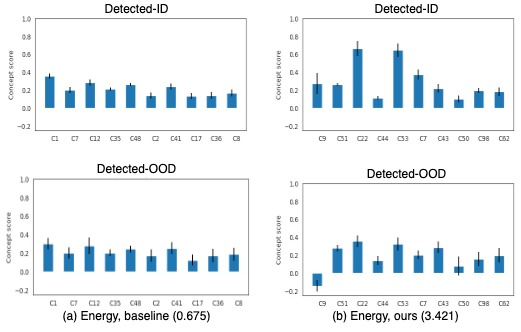
\includegraphics[width=0.8\linewidth]{figures/visual_dstinct.jpg}
  \captionof{figure}{
\small \textbf{Concept separability and visual distinction in the concept score patterns.} For the class "Giraffe", we compare the concept score patterns using two different sets of concepts. \textbf{Left:} Averaged scores of top-10 important concepts out of the concepts learned by ~\cite{yeh2020completeness}). 
\textbf{Right:} Averaged scores of top-10 important concepts out of the concepts learned by our method ($\,\lambda_\textrm{mse} = 1, \lambda_\textrm{norm} = 0.1, \lambda_\textrm{sep} = 50$ with Energy detector).
Concept importance is measured using the Shapley value of Eqn. (\ref{equ: ConceptSHAP}).
% For visualization of what each concept represents, see Appendix.
% C$i$ denotes $i$-th concept.
}
\label{fig:separa_interpretatbility}
\end{figure}

% Lastly, we use the concepts to gain insights on OOD detectors.
% We investigate whether the concepts with a higher concept-separability measure lead to a more distinguishable pattern 
%in the concept scores between detected-ID inputs and detected-OOD inputs. 
% between the concept scores of detected-ID inputs and detected-OOD inputs.
In Fig. \ref{fig:separa_interpretatbility}, we take the average of concept scores $V_{\textrm{in}}(\bfC)$ (or $V_{\textrm{out}}(\bfC)$) among the inputs that are predicted as class $y$, and detected as ID (or OOD) by Energy detector as an example.
% where $\bfC'$ is the subset of original $m$ concepts $\bfC$. 
% Here, we constitute the subset by taking the top-10 important concepts, ranked by their SHAP($\eta^{j}_{\bff, S}(\bfC)$) scores.
% By comparing the patterns of averaged concept scores, one can understand how ID-detected inputs and OOD-detected inputs are different in terms of concepts, even when predicted to same class (compare Figure \ref{fig:low_in} vs. Figure \ref{fig:low_out}, or Figure \ref{fig:high_in} vs. Figure \ref{fig:high_out}).
We can observe noticeably distinguishable pattern between detected-ID and detected-OOD concept scores when using concepts with higher concept separability ($J_{\textrm{sep}}(\bfC, \bfC')=3.421$), compared to those of low concept separability ($J_{\textrm{sep}}(\bfC, \bfC')=0.675$) by ~\cite{yeh2020completeness}. 
These observations confirm our design motivation for the concept separability metric -- that a higher value of the concept separability metric enables better \textit{visual distinction} between the concept score patterns, suggesting better interpretability for humans.
%This suggests that as long as classification completeness and detection completeness are preserved, having higher concept separability is beneficial for better interpretability for humans. 
% For further discussion, see Appendix \ref{sec:appendix-separability}.
\fi

\section{Implementation Details}
\label{sec:appendix-implementation-details}
% In this section, we provide more details about our experiment setting.
We ran all our experiments with Tensorflow, Keras and NVDIA GeForce RTX 2080Ti GPUs. We used test-set bootstrapping with 200 runs to obtain the confidence interval for each hyperparameter setting of concept learning.

\subsection{Experimental Setting.}
\mypara{OOD Datasets.}
For the auxiliary OOD dataset for concept learning ($\Douttr$), we use the unlabeled images from MSCOCO dataset (120K images in total) \cite{lin2014mscoco}. We carefully curate the dataset to make sure that no images contain overlapping animal objects with our ID dataset (\ie 50 animal classes of Animals-with-Attributes \cite{xian2018awa}), then randomly sample 30K images.
For OOD datasets for evaluation ($\Doutte$), we use the high-resolution image datasets processed by Huang and Li~\cite{Huang_MOS}.

\mypara{Hyperparameters for Concept Learning.}
Throughout the experiments, we fix the number of concepts to $m = 100$ (unless specifically mentioned otherwise), and following the implementation of \cite{yeh2020completeness}, we set $\lambda_{\textrm{expl}} = 10$ and $\bfg$ to be a two-layer fully-connected neural network with $500$ neurons in the hidden layer.
We learn concepts based on feature representations from the layer right before the global max-pooling layer of the Inception-V3 model.
% We set the range of $\lambda_{\textrm{norm}}, \lambda_{\textrm{mse}}$ and $\lambda_{\textrm{sep}}$ (in Eqn. (\ref{equ: concept learning})) based on the scale of corresponding regularization terms (\ie $J_{\textrm{norm}}(\bfC, \bfg),  J_{\textrm{mse}}(\bfC, \bfg)$ and $ J_{\textrm{sep}}(\bfC)$, respectively), for a specific choice of the OOD detector.
% For ablation study to illustrate the effect of each parameter, see Appendix \ref{sec:appendix-concept-learning-ablation}.
After concept learning with $m$ concepts, we remove any duplicate (redundant) concept vectors by removing those with a dot product larger than $0.95$ with the remaining concept vectors~\cite{yeh2020completeness}.


\subsection{Additional Results on the Effectiveness of Our Concept Learning}
\label{sec:app_addi_results}

\mypara{Ablation Study for Concept Learning.}
\label{sec:appendix-concept-learning-ablation}
We perform an ablation study that isolates the effect of each regularization term in our concept learning objective (Eqn. \ref{equ: concept learning}) towards our evaluation metrics: classification completeness, detection completeness, and relative concept separability. 
We also observe the coherency among the learned concepts by varying $\lambda_\textrm{mse}$ and $\lambda_\textrm{sep}$.
Coherency of concepts was introduced by Ghorbani \etal~\cite{ghorbani2019ace} to ensure that the generated concept-based explanations are understandable to humans. 
It captures the idea that the examples for a concept should be similar to each other, while being different from the examples corresponding to other concepts.
For the specific case of the image domain, the receptive fields most correlated to a concept $i$ (\eg "stripe pattern") should look different from the receptive fields for a different concept $j$ (\eg "wavy surface of sea").
\citet{yeh2020completeness} proposed to quantify the coherency of concepts as 
\begin{equation}
\label{eq:coherency}
    \frac{1}{m\,K} \mysum_{i=1}^m \mysum_{\bfx^\prime \in T_{\bfc_i}} \langle \bfphi(\bfx^\prime), \bfc_i \rangle,
\end{equation}
where $T_{\bfc_i}$ is the set of $K$-nearest neighbor patches of the concept vector $\bfc_i$ from the ID training set $\Dintr$.

\begin{figure*}[hbt]
  \centering
  \begin{subfigure}{0.45\linewidth}
    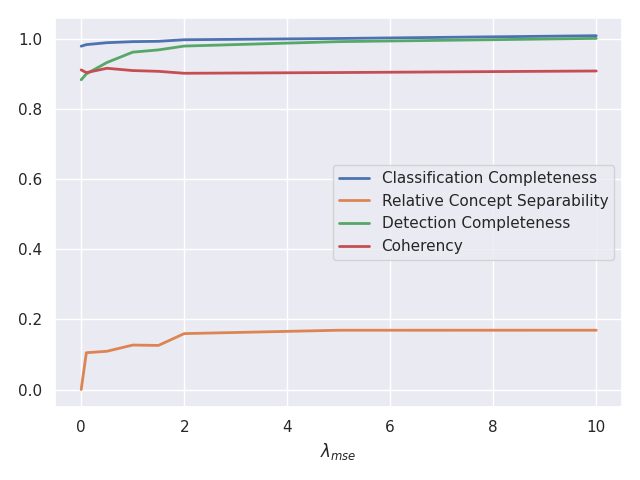
\includegraphics[width=\textwidth]{figures/ablation_mse.png}
    \caption{Ablation study varying $\lambda_\textrm{mse}$; we set $\lambda_\textrm{norm} = 0.1, \lambda_\textrm{sep} = 0$}
    \label{fig:ablation_mse}
  \end{subfigure}
  \hfill
  \begin{subfigure}{0.45\linewidth}
    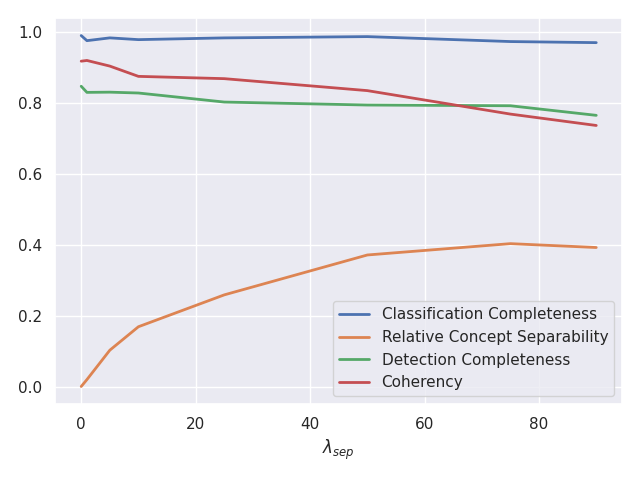
\includegraphics[width=\textwidth]{figures/ablation_sep.png}
    \caption{Ablation study varying $\lambda_\textrm{sep}$; we set $\lambda_\textrm{mse} = 0, \lambda_\textrm{norm} = 0$.}
    \label{fig:ablation_sep}
  \end{subfigure}
  \caption{\textbf{Ablation study with respect to $J_\textrm{mse}(\bfC, \bfg)$ and $J_\textrm{sep}(\bfC)$.} We fix $m = 100, \lambda_\textrm{expl} = 10$, and the OOD detector used for concept learing and evaluation is Energy \cite{liu2020energy}}
\label{fig:ablation}
\end{figure*}

We use this metric to quantify how understandable our concepts are for different hyperparameter choices. Figure~\ref{fig:ablation} shows that aligned with our intuition, large $\lambda_\textrm{mse}$ helps to improve the detection completeness. 
Having non-zero $\lambda_\textrm{mse}$ is also helpful to improve the classification completeness even further, and surprisingly concept separability as well, without sacrificing the coherency of concepts.
On the other hand, on the right side of Figure~\ref{fig:ablation}, we observe that large relative concept separability with large $\lambda_\textrm{sep}$ comes at the expense of lower detection completeness and coherency. 
Recall that when visualizing what each concept represents for human's convenience, we apply threshold 0.8 to only presents (see Figure \ref{fig:app-shap}). 
Low coherency with respect to Eqn. \ref{eq:coherency} (\ie 0.768 with $\lambda_\textrm{sep} = 75)$ means that there is much less number of examples that can pass the threshold, meaning that users can hardly understand what the concepts at hand entail.
This observation suggests that one needs to balance between concept coherency and concept separability depending on which property would be more useful for a specific application of concepts.


\mypara{Effectiveness of the Concept Learning.}
In Table~\ref{tab:concept-learning-results}, we present the complete results of concept learning for various combinations of the regularization coefficients across various real-world, large-scale OOD data: \texttt{Places}, \texttt{SUN} and \texttt{Textures}.

\begin{table*}[htb]
    \centering
    % \begin{adjustbox}{width=1\columnwidth,center}
    \begin{adjustbox}{width=1\textwidth,center}
		\begin{tabular}{l|l|l|c|c|c|c|c|c}
			\toprule
			\multirow{3}{0.001\linewidth}{OOD detector} & \multirow{3}{0.10\linewidth}{Hyper-\\parameters} &
			\multirow{3}{0.05\linewidth}{ $\eta^{}_{\bff}(\bfC) \uparrow$} & \multicolumn{6}{c}{Test OOD dataset} \\ \cline{4-9}
    		& & & \multicolumn{2}{c|}{\texttt{Places}} & \multicolumn{2}{c|}{\texttt{SUN}} & \multicolumn{2}{c}{\texttt{Textures}}\\ \cline{4-9}
    		& & & $\eta^{}_{\bff, S}(\bfC) \uparrow$ & $J_{\textrm{sep}}(\bfC, \bfC') \uparrow$ & $\eta^{}_{\bff, S}(\bfC) \uparrow$ & $J_{\textrm{sep}}(\bfC, \bfC') \uparrow$ & $\eta^{}_{\bff, S}(\bfC) \uparrow$ & $J_{\textrm{sep}}(\bfC, \bfC') \uparrow$ \\ \hline \hline
			%
            \multirow{4}{0.10\linewidth}{MSP} 
			& $(0, 0, 0)$ & 0.977 $\pm$ 0.0006 & 0.774 $\pm$ 0.0010 & 0.694 $\pm$ 0.0153 & 0.782 $\pm$ 0.0010 & 1.088 $\pm$ 0.0175 & 0.593 $\pm$ 0.0013 & 0.765 $\pm$ 0.0157\\
			& $(10, 0.1, 0)$ & \textbf{0.994} $\pm$ 0.0004 & \underline{0.947} $\pm$ 0.0004 & 1.892 $\pm$ 0.0393 & \underline{0.946} $\pm$ 0.0004 & 3.074 $\pm$ 0.0531 & \underline{0.920} $\pm$ 0.0005 & \underline{3.577} $\pm$ 0.1292\\
			& $(0, 0, 50)$ & 0.980 $\pm$ 0.0005 & 0.814 $\pm$ 0.0008 & \underline{2.533} $\pm$ 0.0714 & 0.816 $\pm$ 0.0009 & \underline{4.295} $\pm$ 0.1048 & 0.773 $\pm$ 0.0010 & 3.147 $\pm$ 0.2076\\
			& $(10, 0.1, 50)$ & \underline{0.984} $\pm$ 0.0004 & \textbf{0.960} $\pm$ 0.0004 & \textbf{2.756} $\pm$ 0.0854 & \textbf{0.961} $\pm$ 0.0005 & \textbf{4.442} $\pm$ 0.0830 & \textbf{0.937} $\pm$ 0.0004 & \textbf{3.587} $\pm$ 0.2145\\ \hline
			%
            \multirow{4}{0.10\linewidth}{ODIN} 
			& $(0, 0, 0)$ & 0.977 $\pm$ 0.0006 & 0.742 $\pm$ 0.0011 & 0.444 $\pm$ 0.0119 & 0.745 $\pm$ 0.0010 & 0.710 $\pm$ 0.0156 & 0.618 $\pm$ 0.0013 & 0.501 $\pm$ 0.0121 \\
			& $(10^8, 0.1, 0)$ & \textbf{0.994} $\pm$ 0.0004 & \underline{0.951} $\pm$ 0.0004 & 1.166 $\pm$ 0.0303 & \underline{0.958} $\pm$ 0.0004 & 2.135 $\pm$ 0.0450 & \underline{0.934} $\pm$ 0.0004 & 2.793 $\pm$ 0.0865\\
			& $(0, 0, 50)$ & 0.987 $\pm$ 0.0004 & 0.899 $\pm$ 0.0007 & \underline{1.785} $\pm$ 0.0669 & 0.911 $\pm$ 0.0006 & \underline{3.814} $\pm$ 0.0768 & 0.793 $\pm$ 0.0008 & \underline{3.046} $\pm$ 0.2845\\
			& $(10^8, 0.1, 50)$ & \underline{0.991} $\pm$ 0,0005 & \textbf{0.973} $\pm$ 0.0009 & \textbf{1.813} $\pm$ 0.0268 & \textbf{0.969} $\pm$ 0.0010 & \textbf{4.000} $\pm$ 0.0094 & \textbf{0.945} $\pm$ 0.0006 & \textbf{3.662} $\pm$ 0.1005\\ \hline
			%
            \multirow{4}{0.10\linewidth}{General-ODIN} 
			& $(0, 0, 0)$ & 0.988 $\pm$ 0.0004 & 0.769 $\pm$ 0.0004 & 0.506 $\pm$ 0.0165 & 0.719 $\pm$ 0.0014 & 0.816 $\pm$ 0.0192 & 0.605 $\pm$ 0.0013 & 0.558 $\pm$ 0.1683\\
			& $(10^6, 0.1, 0)$ & \textbf{0.995} $\pm$ 0.0004 & \underline{0.951} $\pm$ 0.0006 & 1.461 $\pm$ 0.0321 & \underline{0.960} $\pm$ 0.0005 & 3.007 $\pm$ 0.0316 & \underline{0.940} $\pm$ 0.0008 & 2.619 $\pm$ 0.1077\\
			& $(0, 0, 50)$ & 0.981 $\pm$ 0.0004 & 0.859 $\pm$ 0.0007 & \underline{1.814} $\pm$ 0.0685 & 0.803 $\pm$ 0.0006 & \underline{4.204} $\pm$ 0.0159 & 0.826 $\pm$ 0.0008 & \textbf{4.014} $\pm$ 0.2246\\
			& $(10^6, 0.1, 50)$ & \underline{0.990} $\pm$ 0.0005 & \textbf{0.971} $\pm$ 0.0010 & \textbf{1.835} $\pm$ 0.0669 & \textbf{0.963}$\pm$ 0.0004 & \textbf{4.287} $\pm$ 0.0284 & \textbf{0.951} $\pm$ 0.0005 & \underline{3.695} $\pm$ 0.1921 \\ \hline
			%
            \multirow{4}{0.10\linewidth}{Energy} 
			& $(0, 0, 0)$ & 0.977 $\pm$ 0.0006 & 0.671 $\pm$ 0.0012 & 0.453 $\pm$ 0.0121 & 0.682 $\pm$ 0.0012 & 0.675 $\pm$ 0.0148 & 0.557 $\pm$ 0.0014 & 0.521 $\pm$ 0.0131\\
			& $(1. 0.1, 0)$ & \textbf{0.993} $\pm$ 0.0005 & \textbf{0.965} $\pm$ 0.0004 & 1.266 $\pm$ 0.0319 & \textbf{0.963} $\pm$ 0.0004 & 2.125 $\pm$ 0.0413 & \textbf{0.960} $\pm$ 0.0003 & 2.648 $\pm$ 0.0596\\
			& $(0, 0, 50)$ & \underline{0.987} $\pm$ 0.0005 & 0.779 $\pm$ 0.0010 & \textbf{1.920} $\pm$ 0.0725 & 0.793 $\pm$ 0.0009 & \textbf{3.659} $\pm$ 0.0659 & 0.767 $\pm$ 0.0010 & \textbf{4.397} $\pm$ 0.2165 \\
			& $(1, 0.1, 50)$ & 0.980 $\pm$ 0.0005 & \underline{0.943} $\pm$ 0.0005 & \underline{1.839} $\pm$ 0.0662 & \underline{0.941} $\pm$ 0.0005 & \underline{3.421} $\pm$ 0.0619 & \underline{0.936} $\pm$ 0.0005 & \underline{3.917} $\pm$ 0.1691 \\ \hline
			%
			\multirow{4}{0.10\linewidth}{Mahala-\\nobis} 
			& $(0, 0, 0)$ & 0.990 $\pm$ 0.0007 & 0.715 $\pm$ 0.0011 & 0.571 $\pm$ 0.0110 & 0.736 $\pm$ 0.0011 & 0.822 $\pm$ 0.0165 & 0.591 $\pm$ 0.0011 & 0.564 $\pm$ 0.0203 \\
			& $(0.1, 0.1, 0)$ & \textbf{0.994} $\pm$ 0.0004 & \underline{0.950} $\pm$ 0.0009 & 1.532 $\pm$ 0.0351 & \underline{0.960} $\pm$ 0.0010 & 2.276 $\pm$ 0.0466 & \underline{0.938} $\pm$ 0.0004 & 2.915 $\pm$ 0.1132\\
			& $(0, 0, 50)$ & 0.985 $\pm$ 0.0004 & 0.880 $\pm$ 0.0005 & \underline{2.550} $\pm$ 0.0681 & 0.883 $\pm$ 0.0006 & \underline{4.091} $\pm$ 0.1013 & 0.774 $\pm$ 0.0007 & \underline{4.274} $\pm$ 0.2305\\
			& $(0.1, 0.1, 50)$ & \underline{0.992} $\pm$ 0.0006 & \textbf{0.961} $\pm$ 0.0005 & \textbf{2.616} $\pm$ 0.0857 & \textbf{0.966} $\pm$ 0.0005 & \textbf{4.325} $\pm$ 0.0055 & \textbf{0.949} $\pm$ 0.0003 & \textbf{4.308} $\pm$ 0.2011 \\ \bottomrule
		\end{tabular}
	\end{adjustbox}
	\caption[]{
	\small \textbf{Results of concept learning with different parameter settings across various OOD detectors and test OOD datasets.} 
% 	$\bfC'$ denotes a set of concepts discovered by baseline \citep{yeh2020completeness} (\ie $\lambda_\textrm{mse} = 0, \lambda_\textrm{norm} = 0, \lambda_\textrm{sep} = 0$).
	Hyperparameters are in the order of $(\lambda_\textrm{mse}, \lambda_\textrm{norm}, \lambda_\textrm{sep})$.
% 	Larger values are better for all the metrics. 
	Across the rows (for a given OOD detector and OOD dataset), the best value is \textbf{boldfaced}, and second best value is \underline{underscored}.
	The $95\%$ confidence intervals are estimated by bootstrapping the test set over $200$ trials.}
% 	\textbf{Bold} numbers indicate the best results (across the rows) for a given OOD detection method and dataset. 
	%Note that by definition of $J_{\textrm{sep}}(\bfC, \bfC')$ (Eqn. \ref{eq:relative-separability}), the relative concept separability of the baseline~\citep{yeh2020completeness} is always $0$, \ie $J_{\textrm{sep}}(\bfC', \bfC') = 0$.
 \label{tab:concept-learning-results}
% \vspace{-.2in}
\end{table*}



\mypara{Accurate Reconstruction of OOD Scores}
In addition to Fig.~\ref{fig:score-distribution-msp}, where we compared the reconstruction accuracy of OOD scores using concepts by \citet{yeh2020completeness} and ours, Fig.~\ref{fig:score-distribution-energy} confirms that the same observation also applies to the Energy detector.

\begin{figure*}
  \centering
  \begin{subfigure}{0.32\linewidth}
    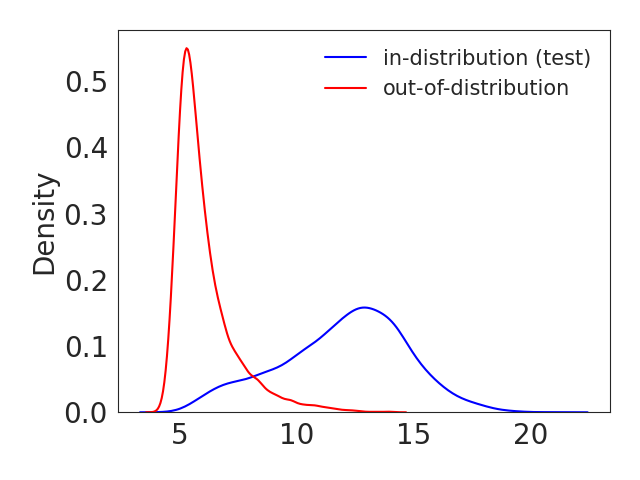
\includegraphics[width=\textwidth]{figures/distr_energy_target.png}
    \caption{\small Empirical distribution of $S(\bfx, \bff)$ from the target detector.}
    \label{fig:short-a1}
  \end{subfigure}
  \hfill
  \begin{subfigure}{0.32\linewidth}
    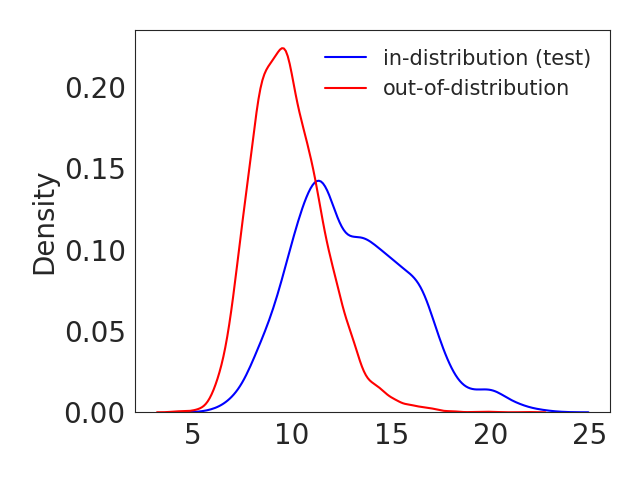
\includegraphics[width=\textwidth]{figures/distr_energy_yeh.png}
    \caption{\small Distribution of $\Scon(\bfx, \bff)$ using concepts learned by \citet{yeh2020completeness}.}
    \label{fig:short-b1}
  \end{subfigure}
  \hfill
  \begin{subfigure}{0.32\linewidth}
    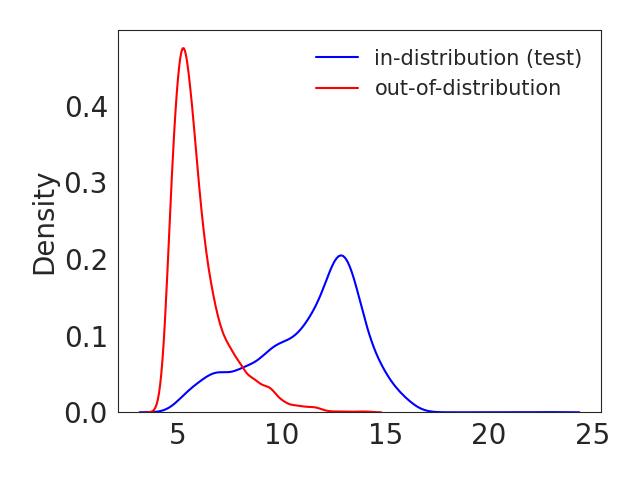
\includegraphics[width=\textwidth]{figures/distr_energy_ours.png}
    \caption{\small Distribution of $\Scon(\bfx, \bff)$ using concepts learned by our method.}
    \label{fig:short-c1}
  \end{subfigure}
  \caption{
  \small (a) Energy detector score $S(\bfx, \bff)$ in the canonical world vs. (b, c) reconstructed $\Scon(\bfx, \bff)$ in the concept world, using different set of concepts.
  Concepts by~\citet{yeh2020completeness} have $\eta^{}_{\bff} = 0.977, ~\eta^{}_{\bff, S}(\bfC) = 0.682$, while concepts by ours $(\lambda_\textrm{mse} = 1, \lambda_\textrm{norm} = 0.1, \lambda_\textrm{sep} = 50)$ have $\eta^{}_{\bff} = 0.984, ~\eta^{}_{\bff, S}(\bfC) = 0.941$.
    Comparison is made between AwA test set (ID, blue) vs. \texttt{SUN} (OOD, red).
    }
\label{fig:score-distribution-energy}
\end{figure*}

\iffalse
\mypara{Transferability of concepts across OOD detectors.}
\label{sec:appendix-concept-learning-transfer}
Our work essentially suggests using a different set of concepts for a specific target OOD detector, as $J_{\textrm{mse}}(\bfC, \bfg)$ and $J_{\textrm{sep}}(\bfC)$ in Eqn. (\ref{equ: concept learning}) depend on a choice of OOD detector. 
In practice, however, one might not have enough computational capacity to prepare multiple sets of concepts for all type of OOD detectors at hand.
Here, we inspect whether the concepts targeted for a certain type of OOD detector are also good to be used for other OOD detectors.
% For instance, 
% $J_\textrm{sep}(\bfC, \bfC') = 0.494$
% But interestingly, relative concept separability tends to be transferred well.
% For full transferability results of concepts targeted for different type of OOD detectors, and tested with different OOD data, see Appendix \ref{sec:appendix-concept-learning-transfer}.

We explore the transferability of concepts targeted to MSP \cite{hendrycks2016msp} detector in Table \ref{tab:transferability-msp}, and Energy \cite{liu2020energy} in Table \ref{tab:transferability-energy}.
Not surprisingly, we observe that concepts targeted for Energy yields the best detection completeness score when tested with the same type of OOD detector, but still make meaningful improvement with other detectors as well.
When it comes to relative concept separability, it is transferred even better across different OOD detectors. 
For instance, the concepts lead to $J_\textrm{sep}(\bfC, \bfC') = 0.862$ with \texttt{Textures}, the best relative concept separability is achieved with ODIN detector (\ie $J_\textrm{sep}(\bfC, \bfC') = 0.862$) and which is even higher than the best results we could obtain using the set of concepts targeted for ODIN (\ie $J_\textrm{sep}(\bfC, \bfC') = 0.414$ with $\lambda_\textrm{mse} = 0, \lambda_\textrm{norm} = 0, \lambda_\textrm{sep} = 50$ in Table \ref{tab:concept-learning-results}).
\begin{table*}[htb]
    % \centering
    % \begin{adjustbox}{}
\begin{subtable}{.47\linewidth}
\begin{adjustbox}{width=\textwidth,center}
\begin{tabular}{l|l|c|c|c|c}
			\toprule
			\multirow{2}{0.35\linewidth}{OOD dataset} & \multirow{2}{0.06\linewidth}{Metrics} & \multicolumn{4}{c}{$\calD$} \\ \cline{3-6}
    		& & MSP & ODIN & Energy & Mahal\\  \hline \hline
    % 		& & & $\mu_{f, \calD} (\bfC)$ & S(\bfC) & $\mu_{f, \calD} (\bfC)$ & S(\bfC) & $\mu_{f, \calD} (\bfC)$ & S(\bfC) & $\mu_{f, \calD} (\bfC)$ & S(\bfC) \\ \hline \hline
			\multirow{2}{0.08\linewidth}{\texttt{Places}} & $\eta^{}_{\bff, S}(\bfC)$ & 0.959 & 0.952 & 0.938 & 0.947\\ 
			& $J_{\textrm{sep}}(\bfC, \bfC')$ & 0.327 & 0.288 & 0.361 & 0.338 \\\hline 
            \multirow{2}{0.08\linewidth}{\texttt{SUN}} & $\eta^{}_{\bff, S}(\bfC)$ & 0.961 & 0.954 & 0.945 & 0.953 \\ 
			& $J_{\textrm{sep}}(\bfC, \bfC')$ & 0.266 & 0.294 & 0.390 & 0.351\\\hline 
			\multirow{2}{0.08\linewidth}{\texttt{Textures}} & $\eta^{}_{\bff, S}(\bfC)$ & 0.938 & 0.946 & 0.932 & 0.930\\ 
			& $J_{\textrm{sep}}(\bfC, \bfC')$ & 0.344 & 0.279 & 0.313 & 0.335\\\hline 
			\multirow{2}{0.08\linewidth}{\texttt{iNaturalist}} & $\eta^{}_{\bff, S}(\bfC)$ & 0.946 & 0.946 & 0.933 & 0.930\\ 
			& $J_{\textrm{sep}}(\bfC, \bfC')$ & 0.286 & 0.181 & 0.229 & 0.197\\
 \bottomrule
    \end{tabular}
    \end{adjustbox}
        \caption[]{Concepts targeted for MSP with $\lambda_\textrm{mse} = 10, \lambda_\textrm{norm} = 0.1, \lambda_\textrm{sep} = 50$}
    \label{tab:transferability-msp}
        \end{subtable}
 % \hfill
     % \small
    % \centering
    \hspace{\fill}
\begin{subtable}{.47\linewidth}
\begin{adjustbox}{width=\textwidth,center}

		\begin{tabular}{l|l|c|c|c|c}
			\toprule
			\multirow{2}{0.35\linewidth}{OOD data} & \multirow{2}{0.06\linewidth}{Metrics} & \multicolumn{4}{c}{OOD detector} \\ \cline{3-6}
    		& & MSP & ODIN & Energy & Mahal\\  \hline \hline
    % 		& & & $\mu_{f, \calD} (\bfC)$ & S(\bfC) & $\mu_{f, \calD} (\bfC)$ & S(\bfC) & $\mu_{f, \calD} (\bfC)$ & S(\bfC) & $\mu_{f, \calD} (\bfC)$ & S(\bfC) \\ \hline \hline
			\multirow{2}{0.08\linewidth}{\texttt{Places}} & $\eta^{}_{\bff, S}(\bfC)$ &0.956& 0.954 &0.971 & 0.954\\ 
			& $J_{\textrm{sep}}(\bfC, \bfC')$ & 0.417 & 0.415 &0.365& 0.410 \\\hline 
            \multirow{2}{0.08\linewidth}{\texttt{SUN}} & $\eta^{}_{\bff, S}(\bfC)$ &0.949& 0.948 &0.970& 0.950\\ 
			& $J_{\textrm{sep}}(\bfC, \bfC')$ & 0.355 &0.286 &0.400& 0.353 \\\hline 
			\multirow{2}{0.08\linewidth}{\texttt{Textures}} & $\eta^{}_{\bff, S}(\bfC)$ &0.931& 0.943 &0.964& 0.947\\ 
			& $J_{\textrm{sep}}(\bfC, \bfC')$ & 0.567 & 0.862&0.494&0.701 \\\hline 
			\multirow{2}{0.08\linewidth}{\texttt{iNaturalist}} & $\eta^{}_{\bff, S}(\bfC)$ &0.943& 0.939 &0.973& 0.940\\ 
			& $J_{\textrm{sep}}(\bfC, \bfC')$ & 0.283 &0.448 &0.280& 0.326\\
 \bottomrule
		\end{tabular}
   
	\end{adjustbox}
        
        \caption[]{Concepts targeted for Energy with $\lambda_\textrm{mse} = 1, \lambda_\textrm{norm} = 0.1, \lambda_\textrm{sep} = 50$}
	\label{tab:transferability-energy}
 \end{subtable}
\caption{Transferability of concepts across different OOD detectors.}
\end{table*}

% \begin{table}[htb]

% \end{table}

\fi 


\subsection{Accurate Reconstruction of Classifier Outputs}
\label{app:hellinger}
We have performed additional experiments to understand if the proposed method can provide improvements in the classification setting. 
Let $\mathbf{C}_1$ denote the concept matrix learned by the method of \citet{yeh2020completeness}. 
Let $\mathbf{C}_2$ denote the concept matrix learned by our method with $\lambda_{mse} = \lambda_{sep} = 0$ and $\lambda_{norm} = 0.1$ (set based on the scale of the regularization term $J_{norm}$). The idea is that we exclude the terms in the concept-learning objective (Eqn.~\ref{equ: concept learning}) that depend on the OOD detector, but include the $\ell_2$ norm based reconstruction error of the layer representation. 
To evaluate the utility of these two sets of concepts for classification, we calculated the per-sample Hellinger distance between the predicted class probabilities of the original classifier and the concept-world classifier (based on either $\mathbf{C}_1$ or $\mathbf{C}_2$). 
Fig.~\ref{fig:hellinger} compares the empirical distribution of the Hellinger distance for both sets of concepts $\mathbf{C}_1$ and $\mathbf{C}_2$. We observe that the distribution is more skewed towards zero with a higher density near zero and a shorter (right) tail in the case of $\mathbf{C}_2$ (red curve) compared to $\mathbf{C}_1$ (blue curve). This suggests that the class predictions are more accurately reconstructed by the concepts learned using our method with only the reconstruction error-based regularization. This can in-turn benefit the concept-based explanations for the classifier.

\begin{figure*}[t]
  \centering
  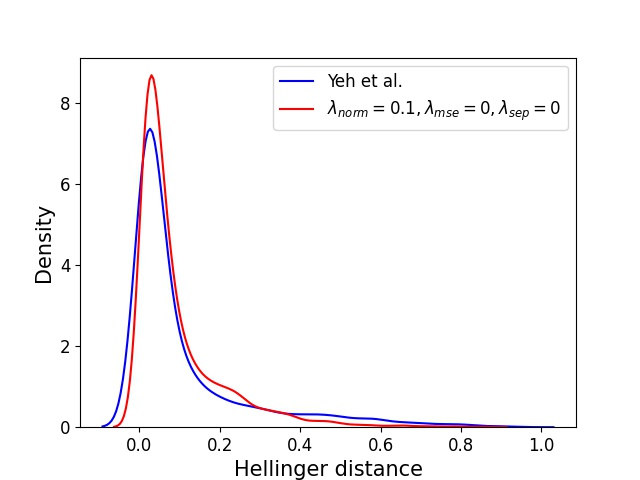
\includegraphics[width=0.5\textwidth]{figures/classification_hellinger.jpg}
\caption{Examples for correct detection}
\label{fig:hellinger}
\end{figure*}


\iffalse

\subsection{Separability in explanations}
\label{sec:appendix-separability}
% Let $X_{in}$ be the set of data detected as ID by $\mathcal{D}$. That is, $\mathcal{D(\bfx)} \geq \tau, ~ \forall \bfx \in X_{in}$. And $X_{out}$ be the set of data detected as OOD by $\mathcal{D}$: $\mathcal{D(\bfx)} < \tau, ~\forall \bfx \in X_{out}$.

% \begin{equation}
%     CAV_{in} = \frac{\sum_{\bfx_i \in X_{in}} v_\bfC(\bfx_i)}{|X_{in}|}
% \end{equation}
% \begin{equation}
%     \label{equ: CAV}
%     CAV_{out} = \frac{\sum_{\bfx_i \in X_{out}} v_\bfC(\bfx_i)}{|X_{out}|}
% \end{equation}

% AwA vs SUN
\begin{figure}[h]
\centering
\subfloat[ID, baseline \label{fig:yeh_low_separa_in}]{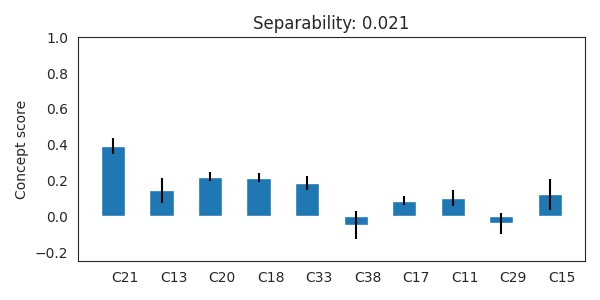
\includegraphics[width=0.5\textwidth]{yeh_class15_AwA2_top10_detected_Energy.jpg}}\hfill
\subfloat[ID, ours \label{fig:ours_low_separa_in}] {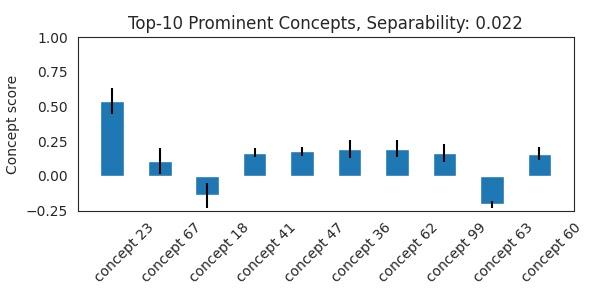
\includegraphics[width=0.5\textwidth]{figures/ours_class15_AwA2_top10_detected_Energy.jpg}}\hfill\\
\subfloat[OOD, baseline\label{fig:yeh_low_separa_out}]{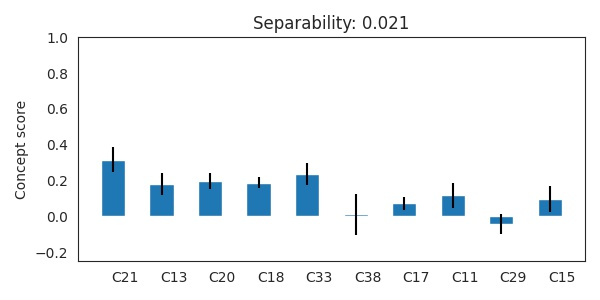
\includegraphics[width=0.5\textwidth]{figures/yeh_class15_SUN_top10_detected_Energy.jpg}}\hfill
\subfloat[OOD, ours \label{fig:ours_low_separa_out}] {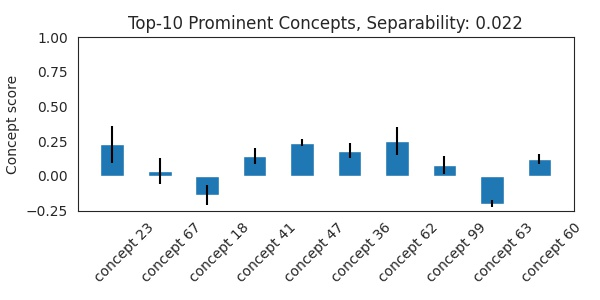
\includegraphics[width=0.5\textwidth]{figures/ours_class15_SUN_top10_detected_Energy.jpg}}
\caption{Easy class ("German Shepherd") with lowest separability. Top-10 concepts with highest conceptSHAP score}
\label{fig:high_separa}
\end{figure}
\fi

\section{Choice of Auxiliary OOD Dataset in Concept Learning}
\label{app:auxiliary-ood}

Under circumstances where having access to auxiliary OOD dataset for concept learning is not feasible, we suggest that one could use generative methods to generate synthetic dataset, or apply data augmentation techniques. Fig.~\ref{fig:app-augAwA} shows an example of AwA image augmented by \citet{hendrycks2022pixmix}. 

\begin{figure*}[hbt]
\centering
{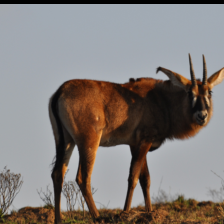
\includegraphics[width=0.2\textwidth]{figures/appendix/9_orig.png}} \hspace{2mm}
{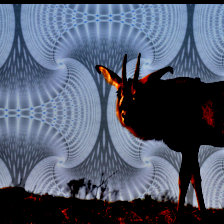
\includegraphics[width=0.2\textwidth]{figures/appendix/9.png}}
\caption{\textbf{Random example of augmented AwA dataset.} 
\textbf{Left:} original image in AwA train set.
\textbf{Right:} corresponding image augmented using the method of \citet{hendrycks2022pixmix}.} 
\label{fig:app-augAwA}
\end{figure*}

We evaluate the effectiveness of our concept learning objective when such augmented AwA train set is used as auxiliary OOD dataset.
Table~\ref{tab:app-auxiliary-ood} illustrates that the generated concepts with augmented AwA (\ie OOD data close to target ID data) have comparable detection completeness and concept separability compared to when MSCOCO (\ie OOD data far from ID data) was used.
But still, further evaluation on generated concept-based explanations with different choice of auxiliary OOD dataset remains as an interesting research question.

\begin{table}[htb]
    \centering
    \begin{adjustbox}{width=1\columnwidth,center}
		\begin{tabular}{l|l|l|c|c|c|c|c|c}
			\toprule
			\multirow{3}{0.001\linewidth}{OOD detector} & \multirow{3}{0.10\linewidth}{Hyper-\\parameters} &
			\multirow{3}{0.05\linewidth}{ $\eta^{}_{\bff}(\bfC) \uparrow$} & \multicolumn{6}{c}{Test OOD dataset} \\ \cline{4-9}
    		& & & \multicolumn{2}{c|}{\texttt{Places}} & \multicolumn{2}{c|}{\texttt{SUN}} & \multicolumn{2}{c}{\texttt{Textures}}\\ \cline{4-9}
    		& & & $\eta^{}_{\bff, S}(\bfC) \uparrow$ & $J_{\textrm{sep}}(\bfC, \bfC') \uparrow$ & $\eta^{}_{\bff, S}(\bfC) \uparrow$ & $J_{\textrm{sep}}(\bfC, \bfC') \uparrow$ & $\eta^{}_{\bff, S}(\bfC) \uparrow$ & $J_{\textrm{sep}}(\bfC, \bfC') \uparrow$ \\ \hline \hline
			%
            % {MSP} & $(10, 0.1, 50)$ & \underline{0.984} $\pm$ 0.0004 & \underline{\textbf{0.960}} $\pm$ 0.0004 & \underline{\textbf{2.756}} $\pm$ 0.0854 & \underline{\textbf{0.961}} $\pm$ 0.0005 & \underline{\textbf{4.442}} $\pm$ 0.0830 & \underline{\textbf{0.937}} $\pm$ 0.0004 & \underline{\textbf{3.587}} $\pm$ 0.2145\\ \hline

            {Energy} 
			& $(1, 0.1, 50)$ & 0.955 $\pm$ 0.0006 & 0.940 $\pm$ 0.0005 & 1.746 $\pm$ 0.0712 & 0.9410 $\pm$ 0.0005 & 3.0703 $\pm$ 0.0580 & 0.927 $\pm$ 0.0005 & 3.417 $\pm$ 0.1419 \\
			\bottomrule
		\end{tabular}
	\end{adjustbox}
        \vspace{2mm}
	\caption[]{Results of concept learning with augmented AwA train set as auxiliary OOD in concept learning.
	}
	\label{tab:app-auxiliary-ood}
\end{table}





\section{Explanations}
\label{sec:appendix-shapleys}


\iffalse
\begin{figure}[h]
% \vspace{1mm}
% \begin{center}
%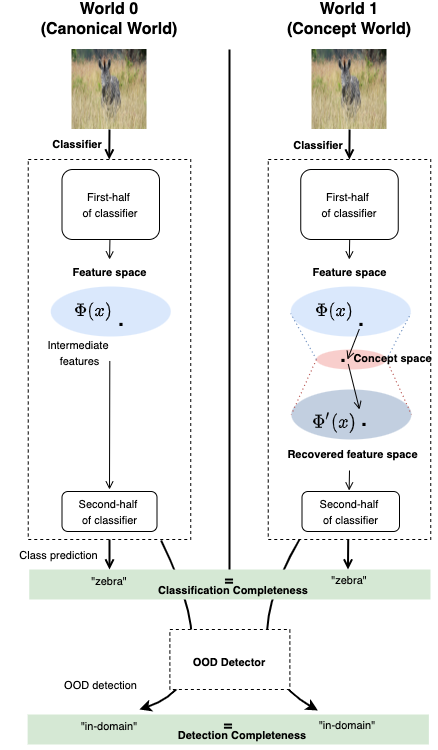
\includegraphics[width=0.45\textwidth]{figures/completeness.png}
% \hspace*{+.5cm} 
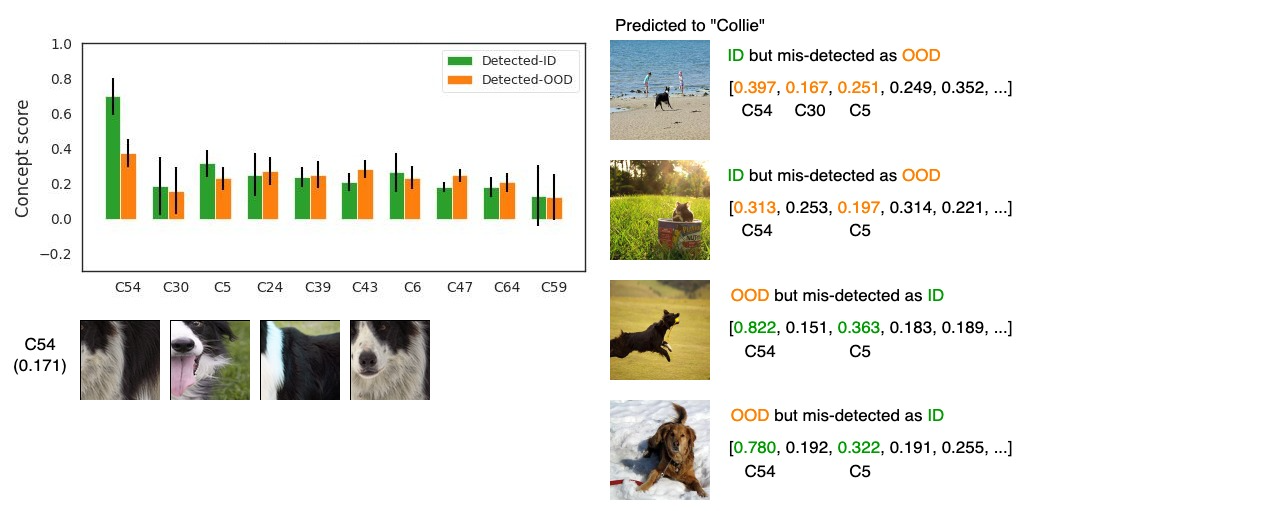
\includegraphics[scale=0.35]{figures/expl_collie.png}
% \vspace{-9mm}
\caption{
\small \textbf{Our concept-based explanations for Energy detector}~\citep{liu2020energy}. Concepts are discovered by our method with $\lambda_\textrm{mse} = 1, \lambda_\textrm{norm} = 0.1, \lambda_\textrm{sep} = 10$.}
\label{fig:expl_collie}
% \end{center}
\end{figure}
\fi

\subsection{Important Concepts for Each OOD Detector}
\label{sec:appendix-explanation}
We show additional examples for the top-ranked concepts by $\textrm{SHAP}(\eta_{\bff, S}, \bfc_i)$ in Fig. \ref{fig:app-shap}.
For each figure with a fixed choice of class prediction, we present receptive fields from ID test set corresponding to top concepts that contribute the most to the decisions of each OOD detector.
All receptive fields passed the threshold test that the inner product between the feature representation and the corresponding concept vector is over $0.85$.
\begin{figure*}[ht]
\centering
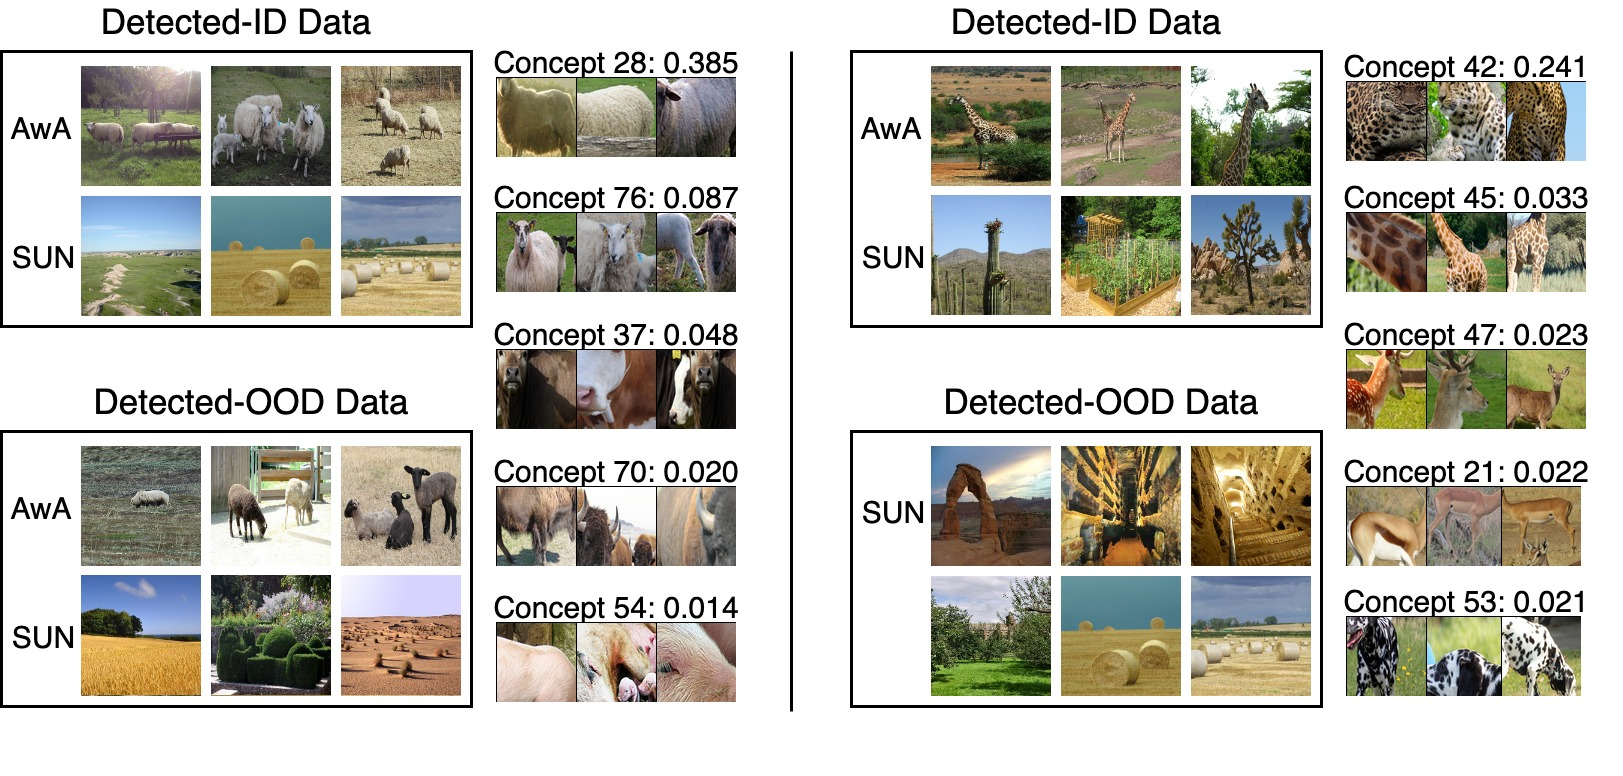
\includegraphics[width=\textwidth]{figures/concepts.jpg}
\vspace{-0.3in}
\caption{Top-6 important concepts for the Energy OOD detector with respect to class ``Sheep'' (on the left) and class ``Giraffe'' (on the right).}
\label{fig:app-shap}
\end{figure*}

Moreover, in Fig. \ref{fig:shap_buffalo}, we compare the important concepts discovered by the baseline method \cite{yeh2020completeness} (denoted as ``baseline'') vs. ours.
With the baseline, when the learned concepts are solely intended for reconstructing the behavior of the classifier, we observe that interpretation of both the classifier and OOD detector depends on a common set of concepts (\ie concepts 32, 10, and 47).
On the other hand, the concepts learned by our method focus on reconstructing the behavior of both the OOD detector and the classifier. In this case, we observe that a distinct set of important concepts are selected for classification and OOD detection.
We also observe that our method requires more concepts in order to address the decisions of both the classifier and OOD detector.
For instance, the number of concepts obtained by our method and the baseline are 78 and 53 (respectively), out of a total 100 concepts after the duplicate removal of concept vectors.
In short, when the concepts are only targeted at explaining the DNN classifier (as in the baseline \cite{yeh2020completeness}), the behavior of the OOD detector is merely described by the common set of concepts that are important for the DNN classifier.
On the other hand, when not only the DNN classifier but also the OOD detector is taken into consideration during concept learning (\ie our method), we obtain a more diverse and expanded set of concepts, and different concepts play a major role in interpreting the classification and detection results. 

\begin{figure}[hbt]
% \vspace{1mm}
\centering
%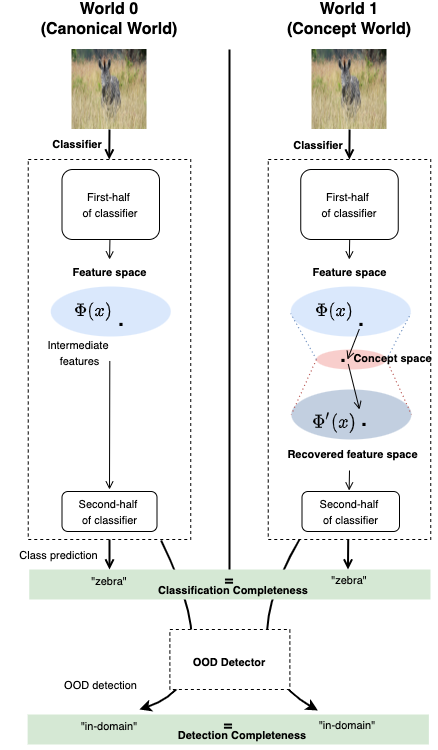
\includegraphics[width=0.45\textwidth]{figures/completeness.png}
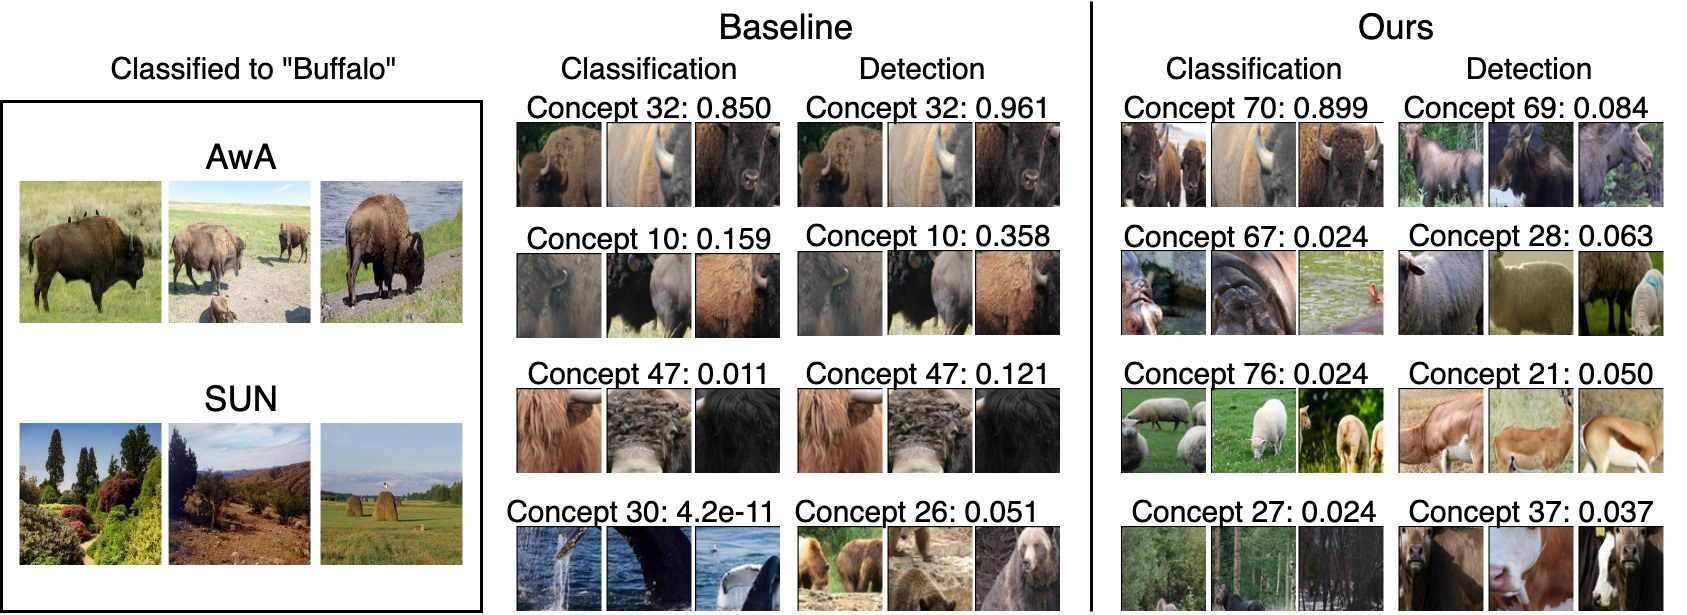
\includegraphics[width=\textwidth]{figures/expl_buffalo.jpeg}
% \vspace{-9mm}
\caption{\textbf{Most important concepts for the Energy detector with respect to the predicted class ``Buffalo''.} 
% Concepts are obtained by our concept learning algorithm with $\lambda_\textrm{mse} = 1, \lambda_\textrm{norm} = 0.1, \lambda_\textrm{sep} = 0$.
We demonstrate randomly sampled images that are predicted by the classifier into this class. 
We compare the top-4 important concepts to describe the DNN classifier (and Energy detector), ranked by the Shapley value based on classification completeness $\textrm{SHAP}(\eta^{j}_{\bff}, \bfc_i)$ (and detection completeness $\textrm{SHAP}(\eta^{j}_{\bff, S}, \bfc_i)$).
``Baseline'' corresponds to the case when the concepts are learned with $\lambda_\textrm{mse} = \lambda_\textrm{norm} = \lambda_\textrm{sep} = 0$, whereas ``Ours'' corresponds to the concepts learned with $\lambda_\textrm{mse} = 1, \lambda_\textrm{norm} = 0.1, \lambda_\textrm{sep} = 0$.
% To visualize what each concept represents, we display the top receptive fields from $\Dinte$ whose inner-product with the corresponding concept vector is larger than 0.8.
}
% \vspace{-5mm}
\label{fig:shap_buffalo}
\end{figure}

\subsection{More Examples of Our Concept-Based Explanation}
\label{app:more-expl}
In Fig.~\ref{fig:expl-additional1}, we provide additional examples of the concept-based explanations provided by  our method and compare it with that of \cite{yeh2020completeness}.

% \textcolor{blue}{Needs a couple of lines about the takeaway message.}



\begin{figure*}[b]
  \centering
  \begin{subfigure}{\linewidth}
    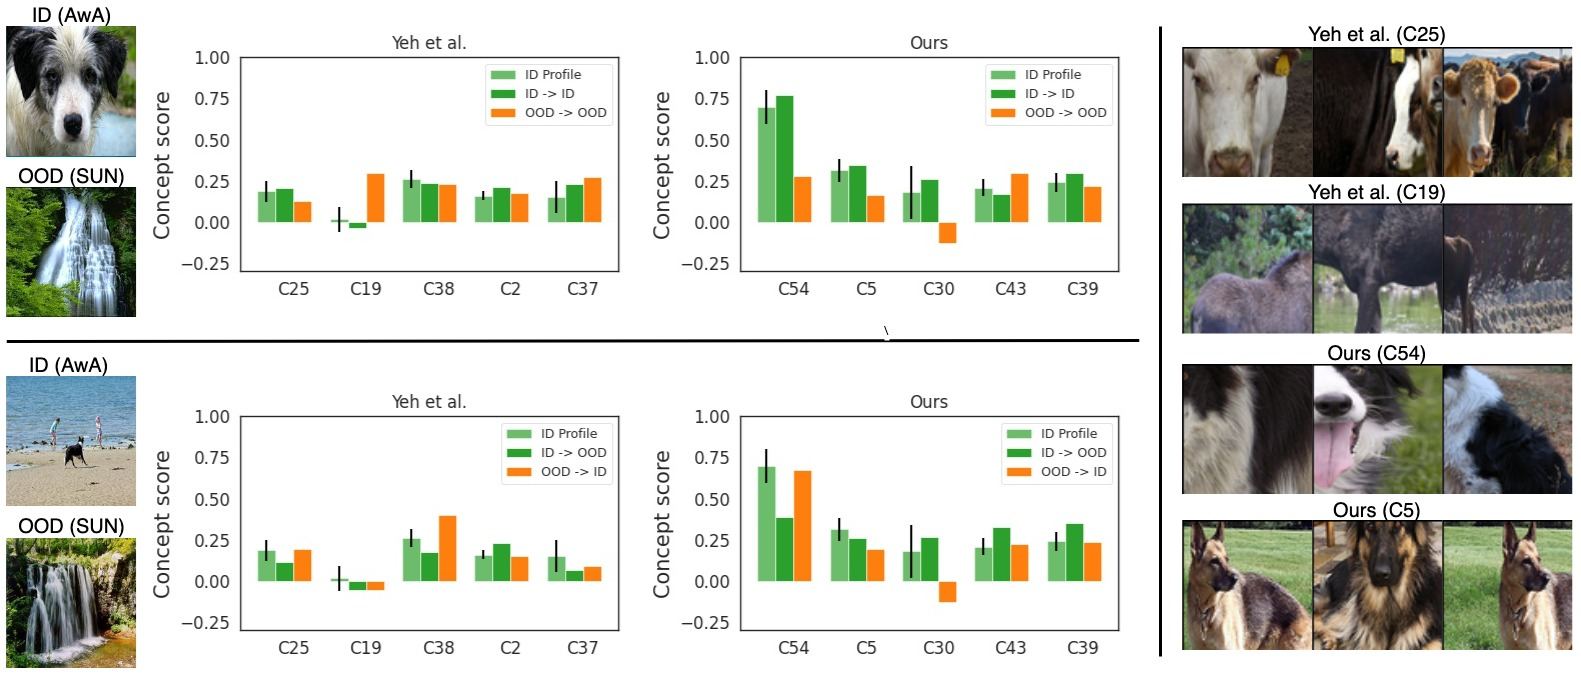
\includegraphics[width=\textwidth]{figures/energy_SUN_Collie.jpg}
    \caption{class ``Collie'', Energy OOD detector. Images randomly selected from AwA test set and \texttt{SUN}.}
    % \label{fig:expl-energy-collie}
  \end{subfigure}
  \\
  \begin{subfigure}{\linewidth}
    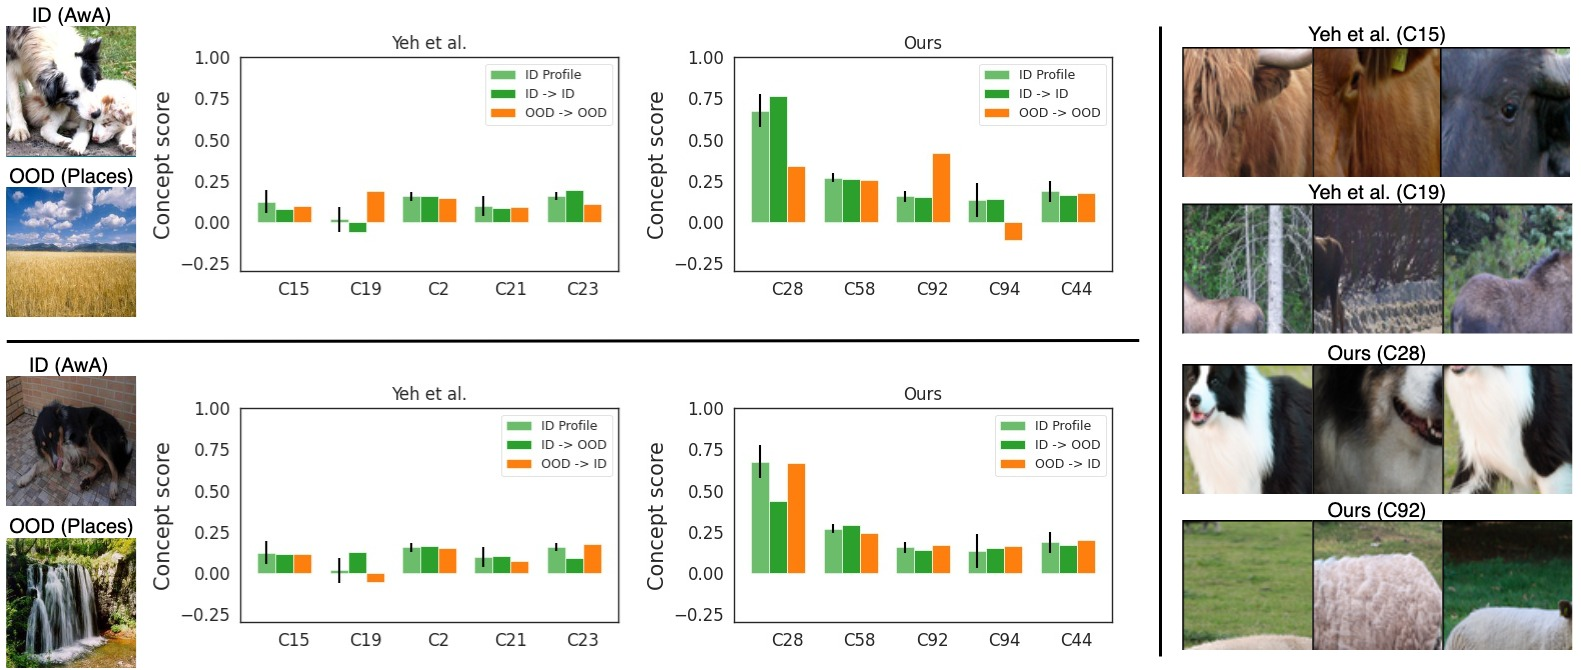
\includegraphics[width=\textwidth]{figures/MSP_SUN_Collie.jpg}
    \caption{class ``Collie'', MSP OOD detector. Images randomly selected from AwA test set and \texttt{SUN}.}
    % \label{fig:expl-energy-collie}
  \end{subfigure}
  % \vspace{.1in}
  % \caption{\textcolor{blue}{\textbf{Concept-based explanations using concepts by Yeh et al. vs. ours.} 
    % ID profile shows the concept-score patterns for normal ID images.}}
\label{fig:expl-additional}
\end{figure*}
  
\begin{figure*}\ContinuedFloat
  \centering
  \begin{subfigure}{\linewidth}
    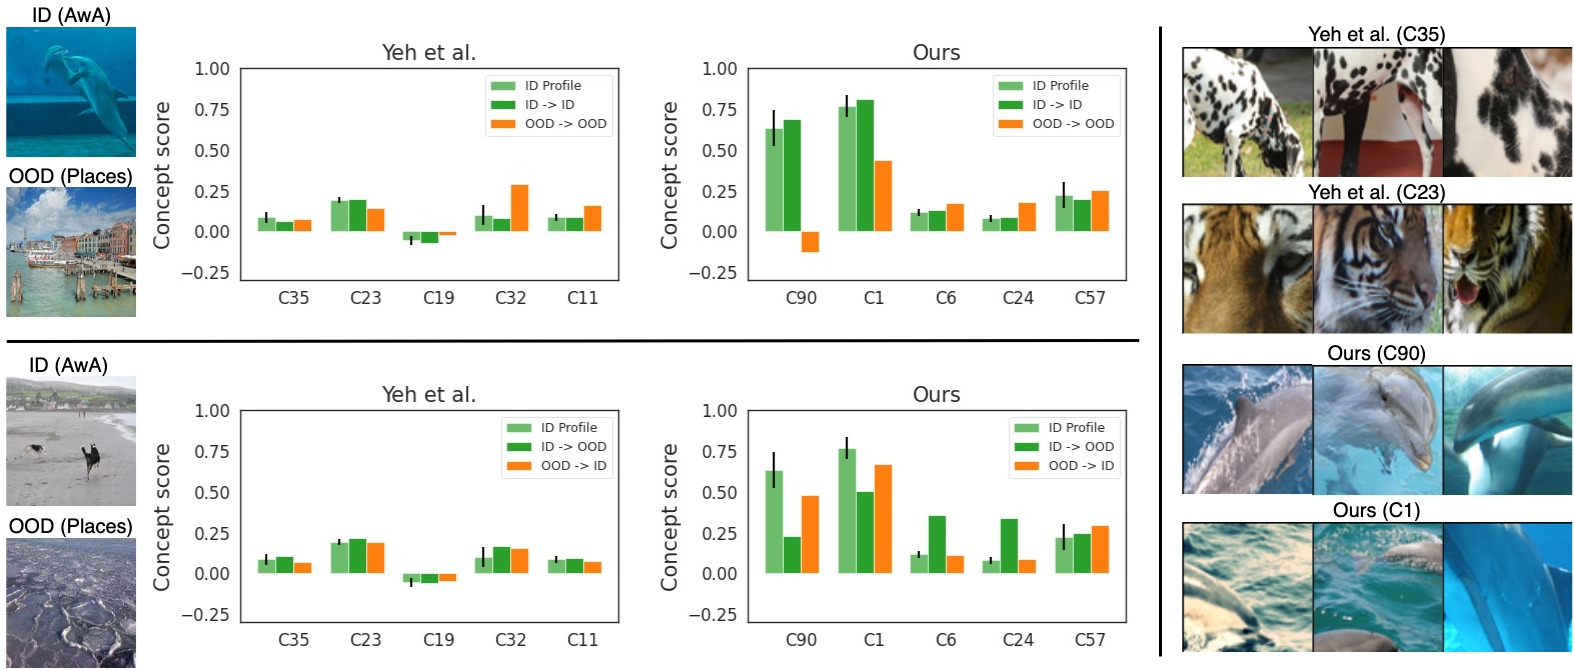
\includegraphics[width=\textwidth]{figures/energy-dolphin.jpg}
    \caption{class ``Dolphin'', Energy OOD detector. Images randomly selected from AwA test set and \texttt{Places}.}
    \label{fig:expl-energy-dolphin}
  \end{subfigure}
  \\
  \begin{subfigure}{\linewidth}
    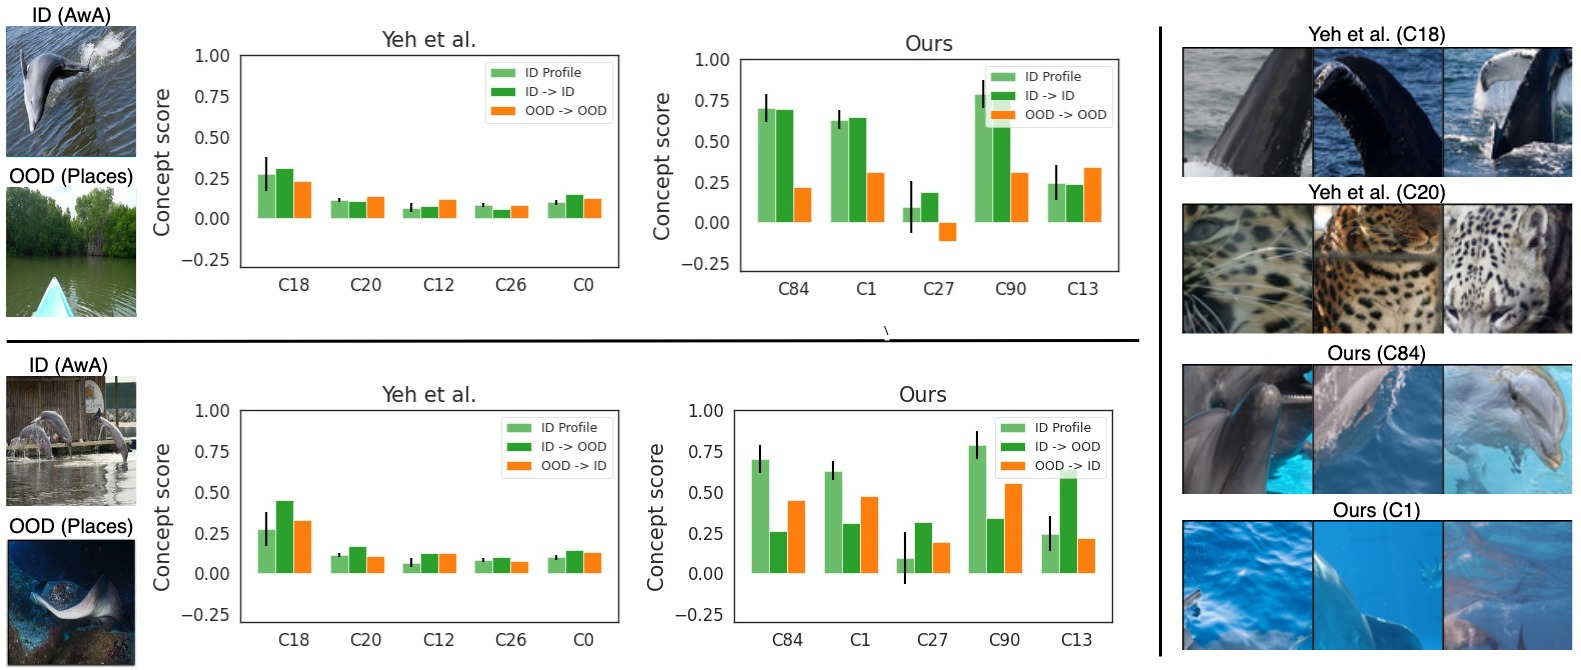
\includegraphics[width=\textwidth]{figures/MSP_Places_Dolphin.jpg}
    \caption{class ``Dolphin'', MSP OOD detector. Images randomly selected from AwA test set and \texttt{Places}.}
    \label{fig:expl-msp-dolphin}
  \end{subfigure}
  \vspace{.1in}
  \caption{\textbf{Concept-based explanations using concepts identified by \citet{yeh2020completeness} vs. ours.}
ID profile shows the average concept-score pattern for normal ID images.}
\label{fig:expl-additional1}
\end{figure*}

\iffalse
\newpage
\subsection{Counterfactual Analysis}
\label{sec:appendix-counterfactual}
% To further verify the contribution of concepts quantified by Eqn. (\ref{equ: ConceptSHAP}), we conduct counterfactual analysis, addressing the following questions: \textit{if the input had these concepts as a dominant features, would it have been detected as ID (or OOD)?}

%
\begin{wrapfigure}{r}{0.5\linewidth}
% \begin{figure}[t]
% \vspace{-10mm}
\centering
%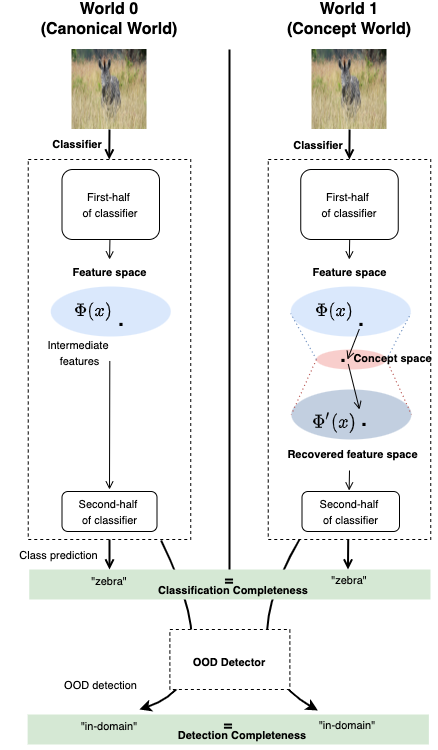
\includegraphics[width=0.45\textwidth]{figures/completeness.png}
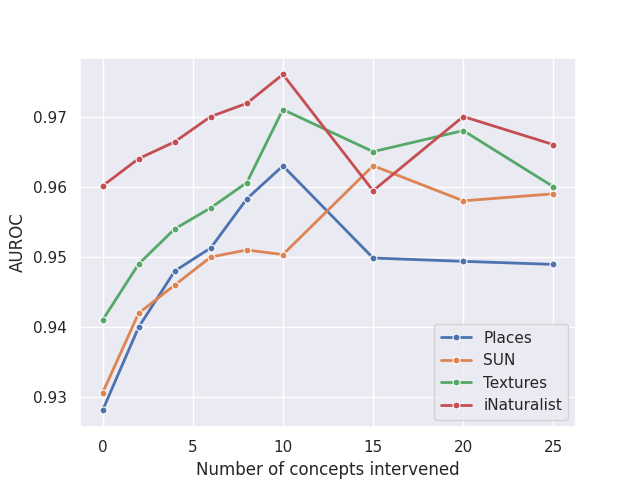
\includegraphics[scale=0.4]{figures/intervention_msp.png}
%\vspace{-2mm}
\caption{Performance of MSP with test-time interventions on concept scoress.}
% \vspace{-5mm}
\label{fig:intervention_msp}
\end{wrapfigure}
% \end{figure}
To verify the important concepts identified by our modified Shapley value, we perform counterfactual analysis, addressing the following question: \textit{if the OOD detector thought the input has different score for this concept, would the detection result be different?}
As we do not assume to have groundtruth annotation for concepts, we construct concept score profiles of detected-ID (or detected-OOD) inputs from held-out ID (or OOD) dataset, and refer to this as ID (or OOD) concept profile.
With the guidance of ID and OOD concept profiles, we take intervention on the concept scores of mis-detected inputs.
Specifically, for ID data mis-detected as OOD, we update their concept scores using ID profiles, and similarlly, for OOD data mis-detected as ID, their concept scores are updated with OOD profiles.
The number of concepts to be intervened can be varied.
As shown in Figure \ref{fig:intervention_msp}, with intervention on more number of important concepts (ranked by $\textrm{SHAP}(\eta^{}_{\bff, S}, \bfc_i)$)), we observe an improved performance of OOD detector in concept world.
\fi

